\chapter{Matrix Element method} \label{ch::MW}

\section{Theoretical framework} \label{sec::MWTheory}
\subsection{MadWeight}

\begin{equation} \label{eq::MWEvtProb}
 P(y \vert a) = \frac{1}{\sigma A} \int
\end{equation}


\subsection{Details on model construction}

\subsection{Optimisations}

Removed the b-jet permutations
\textit{Maybe mention something that a tiny fraction of events is removed due to incomplete reconstruction of the event or due to failing converging (weight = 0). Is the case both on generator and reconstructed level.}

\section{Resolution functions and cross-section normalisaton} \label{sec::TF}
%First of all, the cross-section for these type of events for all the considered coupling coefficients should be determined, which is not as straightforward as was the case for the generator-level events discussed in the previous chapter. The approach opted for in this thesis will be discussed in Section~\ref{sec::RecoAdapt}.

\subsection{Cross-section  normalisation}
\textit{Since it is here a rather general case, first the method for generator-level events can be mentioned and then the difference with reconstructed collision events can be made perfectly clear.}

An important aspect of the Matrix Element method is the normalisation of the event probability using the cross-section and acceptance, which might vary significantly for the considered configurations. For the top-quark mass example given in Section~\ref{sec::TopMass}, the effect of this normalisation was negligible but for the measurement of the anomalous coupling coefficient this factor has proven to be rather important. The method opted for in this analysis to determine these cross-section values will be explained in Section~\ref{subsec::XSReco}.

For the measurement of the right-handed tensor coupling the cross-section normalisation is a vital component.
Independent whether generator-level or reconstructed events are considered, without this normalisation applied the Matrix Element method does not result in the correct outcome.
The substantial influence of this normalisation component has been summarised in Figure~\ref{fig::XSInflGen}, which shows the overall $\chiSqMEM$ distribution prior to and after the cross-section normalisation has been taken into account. The considered sample has been created using the Standard Model configuration such that the minimum of the distribution should correspond to $0$.
%This because the observed variations of the overall event probability for the coupling coefficient are much smaller than was the case for the top-quark mass measurement such that the cross-section normalisation actually has a significant influence on the obtained outcome.
%***********************************
% --> Certain this is the reason?
% ==> Maybe good to think of an explanation why this cross-section normalisation is so much more important
%***********************************
\begin{figure}[h!t]
 \centering
 % Add here the gR gen-level result of FitDistributions_CalibCurve_SemiMu_RgR_AllDeltaTF_MGSampleSM_20000Evts_NoCuts_OuterBinsExclForFit_20000Evts.root with and without XS normalisation
 % Important: Cannot yet use the sample after the event-selection is applied because this still has to be explained!!
 % --> Do this without the fit maybe .. ?
 
\includegraphics[width = 0.3 \textwidth]{image.png} \hspace{0.5cm}
 
\includegraphics[width = 0.3 \textwidth]{image.png}
 \caption{Distribution of the overall $\chiSqMEM$-value obtained by analysing the right-handed tensor coupling using 20 000 generator-level events. The distribution on the left is without any normalisation applied while the right one corresponds to the normalised result.} \label{fig::XSInflGen}
\end{figure}

The significant impact of the cross-section normalisation on the outcome of the measurement implies that the cross-section values for the reconstructed-level analysis should be determined with great care.
However, in contrast to the easy access to generator-level samples with alternative coupling coefficients, generating similar samples containing reconstructed events is a rather challenging and time-consuming process.
As a result, it has been opted for in this thesis to derive the cross-section values for the reconstructed events from the generator-level ones.
This approach significantly facilitates the cross-section determination since any generated process by MadGraph automatically calculates the cross-section of the considered process.
%**********************
% Any other motivation why FastSim has not been considered?
% --> Certain that it would perfectly describe the SM samples??
%**********************
\\
\\
In order to ensure that the obtained generator-level cross-sections can easily be related to the reconstructed ones, the conditions present for the reconstructed collision events will be mimicked as closely as possible during the generation process. Hence the generator events have to fullfill the basic event selection requirements\footnote{Important to note here is that once these selection criteria are applied to the generated events, the obtained cross-section will actually be a combination of the cross-section of the underlying physics process and the acceptance of the considered event selection. Hence the term ``cross-section normalisation'' will \textbf{implicitely} imply the combined normalisation $\sigma \times A$ mentioned in Equation~\ref{eq::MWEvtProb}.} listed in Table~\ref{table::GenCuts}.
By applying a significant fraction of the full event selection chain onto the generated events, the expected relative difference in behaviour of each $\gR$ value on the considered kinematic constraints will be incorporated. As previously mentioned in Section~\ref{sec::CalibCurve}, the remaining event-selection criteria are supposed to be less sensitive to the value of the coupling coefficient.
%The remaining event selection criteria are believed to be less sensitive to the value of the coupling coefficient, thus their relative dependence will not be taken into account.
\\
\\
In addition, the generated processes are also selected in order to remain with a similar event signature as is the case in data. Hence the cross-section values have been determined using a combination of top-quark pair decay processes surrounded with additional jets. The actual number of considered processes has been limited to the $\ttbar$ decay with none, one and two additional jets since the contribution of the following decays quickly becomes negligible.
%********************************************
% --> Does this correspond to LO, NLO and NNLO or is this still something different??
% Question: Interesting to give some of the Feynman diagrams belonging to the different processes?
%********************************************
\begin{figure}[h!t]
 \centering
 
\includegraphics[width = 0.15 \textwidth]{image.png} \hspace{0.2cm}
 
\includegraphics[width = 0.15 \textwidth]{image.png} \hspace{0.2cm}
 
\includegraphics[width = 0.15 \textwidth]{image.png}
 \caption{Feynman diagrams for the different generator-level processes considered for the calculation of the cross-sections. \textbf{Relevant?}}
\end{figure}

Even with these two optimisations applied, this approach will not result in a perfect agreement with the selected events. For instance, it is simply not possible to include every aspect of the full event-selection chain in exactly the same way when generating the different processes.
Hence, the obtained cross-section values will be scaled in order to take into account the influence of these non-included event selection criteria.
For this an identical behaviour throughout the entire $\gR$ range is assumed such that each cross-section value will be multiplied with the factor $\sigma_{SM}^{reco}$/$\sigma_{SM}^{gen}$. 
%********************************************
% --> Think of any other non-included effects!!
%********************************************
\\
In this factor the term $\sigma_{SM}^{reco}$ represents the measured cross-section of the selected events while the cross-section obtained for the combined generator-level sample created using the Standard Model configuration is denoted by $\sigma_{SM}^{gen}$.
The cross-section of the selected events is determined by dividing the semi-leptonic $\ttbar$ event count obtained after the full event selection chain with the luminosity of this sample, which has been given previously in Table~\ref{table::Samples}. 
\\

The final result of the cross-section calculation can be found in Figure~\ref{fig::XSDistr}, which shows the distribution of the cross-section values obtained for the generator-level events using the approach discussed above. The cross-section values for the selected events are also given in this Figure, obtained by multiplying each of the former cross-sections with the fixed scaling factor $\sigma_{SM}^{reco}$/$\sigma_{SM}^{gen}$ = $0.134$.
\\
\textbf{Remark: Used luminosity and number of events do not seem to be correct!}
\begin{figure}[h!t]
 \centering
 \includegraphics[width = 0.7 \textwidth]{Chapters/Chapter6_Analysis/Figures/XSDistributions.pdf}
 \caption{Overview of the distribution of the generator-level cross-sections for different $\gR$ values and the reconstructed ones derived from them by applying the ratio $\sigma_{SM}^{reco}$/$\sigma_{SM}^{gen}$.} \label{fig::XSDistr}
\end{figure}

%--------------------------------------------------------------------------------------------------------- \\
%Also here there is an additional complexity when considering reconstructed events, since the cross-section of the $\ttbar$ decay depends on the value of the coupling coefficients in the interaction vertex. For generator-level events, these values are accesible for each generated sample since MadGraph automatically determines the cross-section of each generated process.
%\\
%Hence the cross-sections for these reconstructed events are derived from the MadGraph predictions by carefully calculating the generator-level cross-sections in a regime comparable to data. 
%This condition has been achieved by combining the cross-sections for each $\gR$ coefficients when no, one and two additional jets are included in the event. 
%This will not result in a perfect match to data, but will bring the considered configuration a bit closer to reality. 
%\\
%Since the cross-section should be include the effect of the event selection, the different MadGraph samples have to fullfill the different kinematic requirements given in Table~\ref{table::GenCuts}. The three different contributions are then added in order to obtain an overall cross-section for the \textbf{inclusive} 2-jet case, for which the results have been summarised in the second column of Table~\ref{table::XSValues}.
%The third column contains the cross-section values that will be applied for the measurement using the reconstructed events, and have been obtained by scaling the cross-section for each $\gR$ value with the fraction $\sigma_{SM}^{reco}$/$\sigma_{SM}^{gen}$. This ratio corrects the generator-level cross-sections to the expected reco-level one and can be applied onto all $\gR$ configurations since the relative effect of the event selection is already been incorporated by applying the basic event selection requirements on the MadGraph samples. The value $\sigma_{SM}^{reco}$ has been determined by dividing the number of selected events with the total number of events present in the sample and multiplying this with the cross-section of the semi-leptonic $\ttbar$ sample, which thus corresponds to multiplying the selected number of events with the luminosity of the simulated sample. The distribution of the generator-level cross-sections and the reconstructed ones is given in Figure~\ref{fig::XSDistr} and serves as an easy way to determine the reconstructed cross-section for other $\gR$ values if required.
%
%\begin{table}[h!t]
%  \centering
%  \caption{Overview of the cross-section values used for the reconstructed events together with the inclusive $\ttbar$+2jet events from which they have been derived. \textbf{Maybe redundant if figure is %given ..}} \label{table::XSValues}
%  \small
%  %\begin{tabular}{|c||c|c|c|c||c|}
%  \begin{tabular}{|c|c|c|}
%   \hline
%%   $\gR$ coefficient 	& $\ttbar$+0j ($\pbinv$) 	& $\ttbar$+1j ($\pbinv$) 	& $\ttbar$+2j ($\pbinv$) 	& Incl. $\ttbar$+2j 	& $\ttbar$ reco ($\pbinv$) 	\\
%   $\gR$ coefficient 	& Incl. $\ttbar$ + 2 jets ($\pbinv$) 	& $\ttbar$ reco ($\pbinv$) 	\\
%   \hline
%   \hline
%   -0.2  		& 3.34036				& 0.947244 			\\
%   -0.15		& 4.01717				& 1.13624			\\
%   -0.1 		& 4.84056				& 1.36448			\\
%   -0.05		& 5.82329 				& 1.63952			\\
%   0.0 		& 6.98981 				& 1.96892			\\
%   0.05		& 8.37733 				& 2.36027			\\
%   0.1 		& 10.0153 				& 2.82111			\\
%   0.15		& 11.9024 				& 3.35903			\\
%   0.2 		& 14.0873 				& 3.98157			\\
%   \hline
%  \end{tabular}
%\end{table}

\subsection{Resolution functions}


\paragraph{Update of Friday 16 October 2015 :} 
Important issue about the Transfer Functions discovered by looking at their distribution beyond the fitted range!
\\

The way the TF's were determined was by optimizing the fitted range and making sure that the fit corresponded well with the measured MC points. However this way there is no control about what happens beyond this range, and looking at the full fit function clearly indicated strange shapes and peaks in this area. This was also neatly visible in the comparison of the ``old'' and ``new'' TF's (b-jets mainly). 
\\
\textit{ \underline{Remark: } The strange behaviour of the ``old'' TF is not really understood. When looking at the individual fit distributions when creating these shapes the minimum was always positioned at the expected position.}
\begin{figure}[h!t]
 \centering
 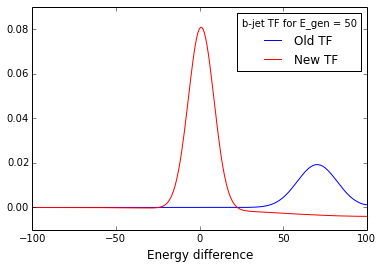
\includegraphics[width = 0.24 \textwidth]{Chapters/Chapter5_MadWeight/Figures/BJetTF_OldvsNew_Egen50.png}
 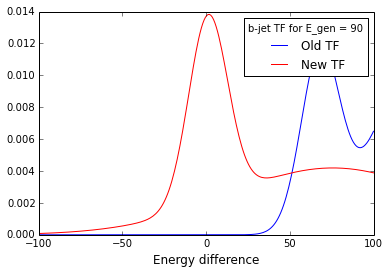
\includegraphics[width = 0.24 \textwidth]{Chapters/Chapter5_MadWeight/Figures/BJetTF_OldvsNew_Egen90.png}
 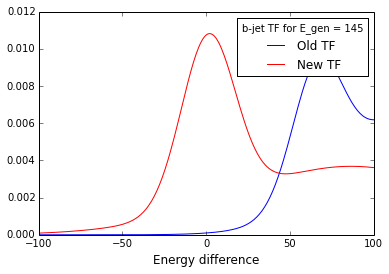
\includegraphics[width = 0.24 \textwidth]{Chapters/Chapter5_MadWeight/Figures/BJetTF_OldvsNew_Egen145.png}
 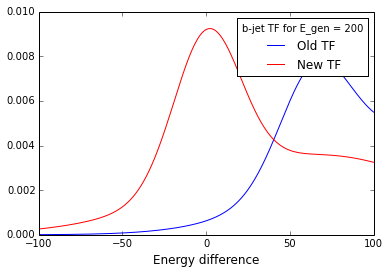
\includegraphics[width = 0.24 \textwidth]{Chapters/Chapter5_MadWeight/Figures/BJetTF_OldvsNew_Egen200.png}
 \caption{Comparison between the old (blue) and new (red) TF in order to understand why the former does give the correct minimum and the latter one not. From these plots a conclusion cannot really be made since it seems that none of them actually corresponds to the expected distribution. For the most recent one the additional peak at positive $\Delta E$ values should clearly dissapear.}
\end{figure}
\hfill \\
For this reason the method to determine the TF's has been adapted such that the full fit function is visible and not only the fit on the restricted range. In order to better visualize the tail and the double gaussian behaviour further from 0, the considered $\Delta E$ range has also been extended up to $-100$ and $100$. 
\\
This new approach indicates that the old method gave rise to completely wrong distributions and that the only way to capture the tail is by giving up the precise determination of the peak a little bit. For each of the $E_{gen}$ bins of the b-jet distribution the position of the main peak is slightly off, but in general the shape can be labelled acceptable (and results in decent parameter results).
\begin{figure}[h!t]
 \centering
 \includegraphics[width = 0.49 \textwidth]{Chapters/Chapter5_MadWeight/Figures/sliceYbin1And2_BJet_DiffEVsGenE.pdf}
 \includegraphics[width = 0.49 \textwidth]{Chapters/Chapter5_MadWeight/Figures/sliceYbin8_BJet_DiffEVsGenE.pdf}
 \includegraphics[width = 0.49 \textwidth]{Chapters/Chapter5_MadWeight/Figures/sliceYbin1And2_BJet_DiffEVsGenE_OLDRange.pdf}
 \includegraphics[width = 0.49 \textwidth]{Chapters/Chapter5_MadWeight/Figures/sliceYbin8_BJet_DiffEVsGenE_OLDRange.pdf}
 \caption{Upper plots are obtained with the new method (focus on shape outside fitted range) while lower ones are how the TF were created earlier (focus on good fit in range).}
\end{figure}
\hfill \\
When comparing these new TF's with the old ones, the strange shape on the positive side of $\Delta E$ completely dissapeared and now looks more like the expected distribution.
\begin{figure}[h!t]
 \centering
 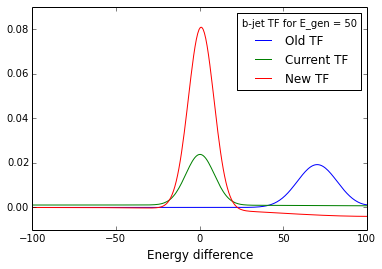
\includegraphics[width = 0.24 \textwidth]{Chapters/Chapter5_MadWeight/Figures/BJetTF_OldvsNewvsCurr_Egen50.png}
 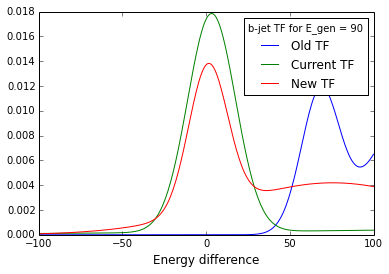
\includegraphics[width = 0.24 \textwidth]{Chapters/Chapter5_MadWeight/Figures/BJetTF_OldvsNewvsCurr_Egen90.png}
 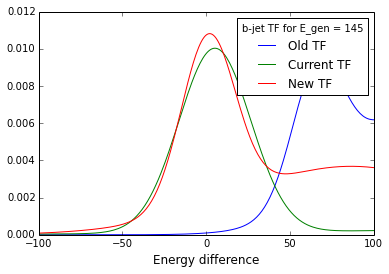
\includegraphics[width = 0.24 \textwidth]{Chapters/Chapter5_MadWeight/Figures/BJetTF_OldvsNewvsCurr_Egen145.png}
 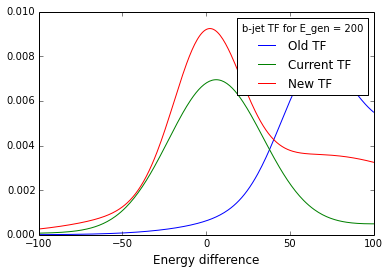
\includegraphics[width = 0.24 \textwidth]{Chapters/Chapter5_MadWeight/Figures/BJetTF_OldvsNewvsCurr_Egen200.png} 
 \caption{Overall distribution obtained for the new TF's for different $E_{gen}$ energies.}
\end{figure}
\hfill \\
To finalize the TF discussion for the b-jets, the obtained parameter distributions are given. These represent the obtained mean and width of the two gaussians and their relative weight in the fit formula. The results look rather stable, beside some fluctuations for the wide gaussian, which is also expected since this one can be determined not as precise as the narrow one. However the $E_{gen}$ bins where the wide gaussian is expected to be more important succeeded in measuring the required precise enough to do the fit. 
\\
The most thrustworthy result is obtained for the relative constant which clearly shows that the second gaussian only becomes significant for higher values of $E_{gen}$ since the $\Delta E$ distribution becomes significantly broader for these events. However it is also the region where the double gaussian shape matches best with the fitted MC points.
\begin{figure}[h!t]
 \centering
 \includegraphics[width = 0.32 \textwidth]{Chapters/Chapter5_MadWeight/Figures/BJet_DiffEVsGenE_a1_Fit.pdf}
 \includegraphics[width = 0.32 \textwidth]{Chapters/Chapter5_MadWeight/Figures/BJet_DiffEVsGenE_a2_Fit.pdf}
 \includegraphics[width = 0.32 \textwidth]{Chapters/Chapter5_MadWeight/Figures/BJet_DiffEVsGenE_a3_Fit.pdf}
 \includegraphics[width = 0.32 \textwidth]{Chapters/Chapter5_MadWeight/Figures/BJet_DiffEVsGenE_a4_Fit.pdf}
 \includegraphics[width = 0.32 \textwidth]{Chapters/Chapter5_MadWeight/Figures/BJet_DiffEVsGenE_a5_Fit.pdf}
\end{figure}

For some (currently unexplained) reason the result obtained for the light jets did not encounter the same issue and here the distributions for the ``old'' and ``new'' TF's were almost identically. Hence only effort has been awarded to the b-jet fixing in order to run a quick test whether this would already result in the expected outcome.
\begin{figure}[h!t]
 \centering
 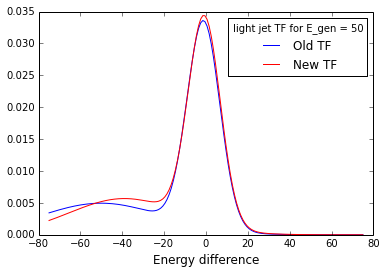
\includegraphics[width = 0.3 \textwidth]{Chapters/Chapter5_MadWeight/Figures/LightTF_OldvsNew_Egen50.png}
 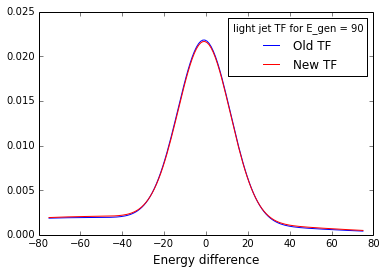
\includegraphics[width = 0.3 \textwidth]{Chapters/Chapter5_MadWeight/Figures/LightTF_OldvsNew_Egen90.png}
 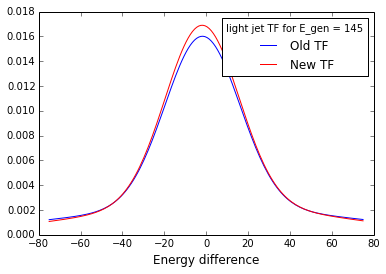
\includegraphics[width = 0.3 \textwidth]{Chapters/Chapter5_MadWeight/Figures/LightTF_OldvsNew_Egen145.png}
 \caption{Comparison of TF's for the light jets, which are clearly almost identical. Hence no update for these has been done for the moment.}
\end{figure}
\hfill \\
In order to be sure the light jets really behave properly, some examples of individual fit distributions have been added anyway. This indeed shows that the double Gaussian shape correctly takes both the peak and the tail. However some minor improvement can still be achieved in the negative side of the $\Delta E$ distribution for low values of $E_{gen}$. As a final cross-check the range of the muon distributions will also be extended up to $-75$ and $75$ in order to check whether some improvement can be reached, as was the case for the b-jet distributions.
\begin{figure}[h!t]
 \centering
 \includegraphics[width = 0.49 \textwidth]{Chapters/Chapter5_MadWeight/Figures/sliceYbin1And2_Light_DiffEVsGenE.pdf}
 \includegraphics[width = 0.49 \textwidth]{Chapters/Chapter5_MadWeight/Figures/sliceYbin8_Light_DiffEVsGenE.pdf}
 \caption{Fit distributions for light jets which again indicate that the original method works out-of-the-box for the light jets and do not experience the same strange behaviour as the b-jets.}
\end{figure}

For the moment, to quickly check the influence of these updated b-jet TF's, it has been decided to use delta-functions for the muons. However looking at the narrow $\Delta E$ distributions for the muon events, it is maybe sufficient to use delta-functions for the actual analysis.
%As a final remark, it has been decided to use delta-functions for the muons since this will be good enough. (Also paper of Kelly goes out with delta for muons and this will be made public...). 
In case electrons would be considered this however requires non-delta shaped TF's.\\
If really necessary the same procedure can be done in order to provide eta-binned TF's for both the b-jets and the light jets, but this will again require a lot of time ... And as long als the final TF's haven't been decided on, the full list of MC samples cannot be send through MadWeight!

\section{Matrix Element method in practice}
\subsection{Extracting information from the likelihood}
\subsection{Determining the top-quark mass using the Matrix Element method}
Sample created using 4000 correct semi-leptonic $\ttbar$ events.
